\documentclass[11pt]{beamer}
\usetheme{Singapore}

\usepackage[utf8]{inputenc}
\usepackage[T1]{fontenc}
\usepackage{soul}
\usepackage{graphicx}


\graphicspath{{../../Figures/}}

\def\et{{\it et al.}}


\author{Cody Glickman \\ CPBS Update Talk}

\title{Metagenomic Exploration: \\ Evaluation and development of novel tools for viral and bacterial sequence analysis}

%\subtitle{}
%\logo{}

\date{ 
\includegraphics[height=2cm, width=2cm]{lablogo.png} \\ Jan 29th, 2018}
%\subject{}
\setbeamercovered{transparent}
\setbeamertemplate{navigation symbols}{}
\setbeamertemplate{theorems}[numbered]

\begin{document}
	\maketitle
	\begin{frame}{Research Update}
	\begin{block}{Asthma Environmental Microbiome}
	\end{block}
	\vspace{-0.5cm}
	\begin{block}{\alert{Building Up Domains}}
	\end{block}
	\vspace{-0.5cm}
	\begin{block}{Clinical Features of Cystic Fibrosis and the Microbiome}
	\end{block}
	\vspace{-0.5cm}
	\begin{block}{\alert{Genomic Retrieval and Blast Database Creation}}
	\end{block}
	\vspace{-0.5cm}
	\begin{block}{Hawaiian Soil Chemistry and Culture}
	\end{block}
	\vspace{-0.5cm}
	\begin{block}{Microbiome OTU Grouping Workflow}
	\end{block}
	\vspace{-0.5cm}
	\begin{block}{\alert{Metagenomic Simulation Study}}
	\end{block}
	\vspace{-0.5cm}
	\begin{block}{Virome Statistics Pipeline}
	\end{block}
	\end{frame}
	
	
\section{Introduction}
\subsection{}

	\begin{frame}{Nontuberculous Mycobacterial (NTM) Infections}
		\begin{block}{Number of Cases}
		The number of NTM cases is estimated over 100K
		\end{block}
		
		\begin{block}{Increasing Case}
		The rate of cases is estimated to grow at 8\% every year
		\end{block}
		
		
		\begin{block}{Populations at risk of developing NTM}
		\begin{itemize}
		\item Immunocompromised individuals 
		\item Patients with lung damage or malfunction 
		\item Residents of warm costal areas especially Hawaii
		%\item The Elderly 
		\end{itemize}
		\end{block} 
		
		\begin{block}
		
		\end{block}
	\vspace{-1cm}
	\tiny{Strollo SE, et al. Ann Am Thorac Soc. 2015 \\
	Adjemian J, et al. Am J Respir Crit Care Med. 2012}
	
	\end{frame}
	
	\begin{frame}{Understanding Why NTM Develops}
	\begin{block}{Hawaiian Soil Project}
	Identifying important soil characteristics for NTM soil culture 
	\center
	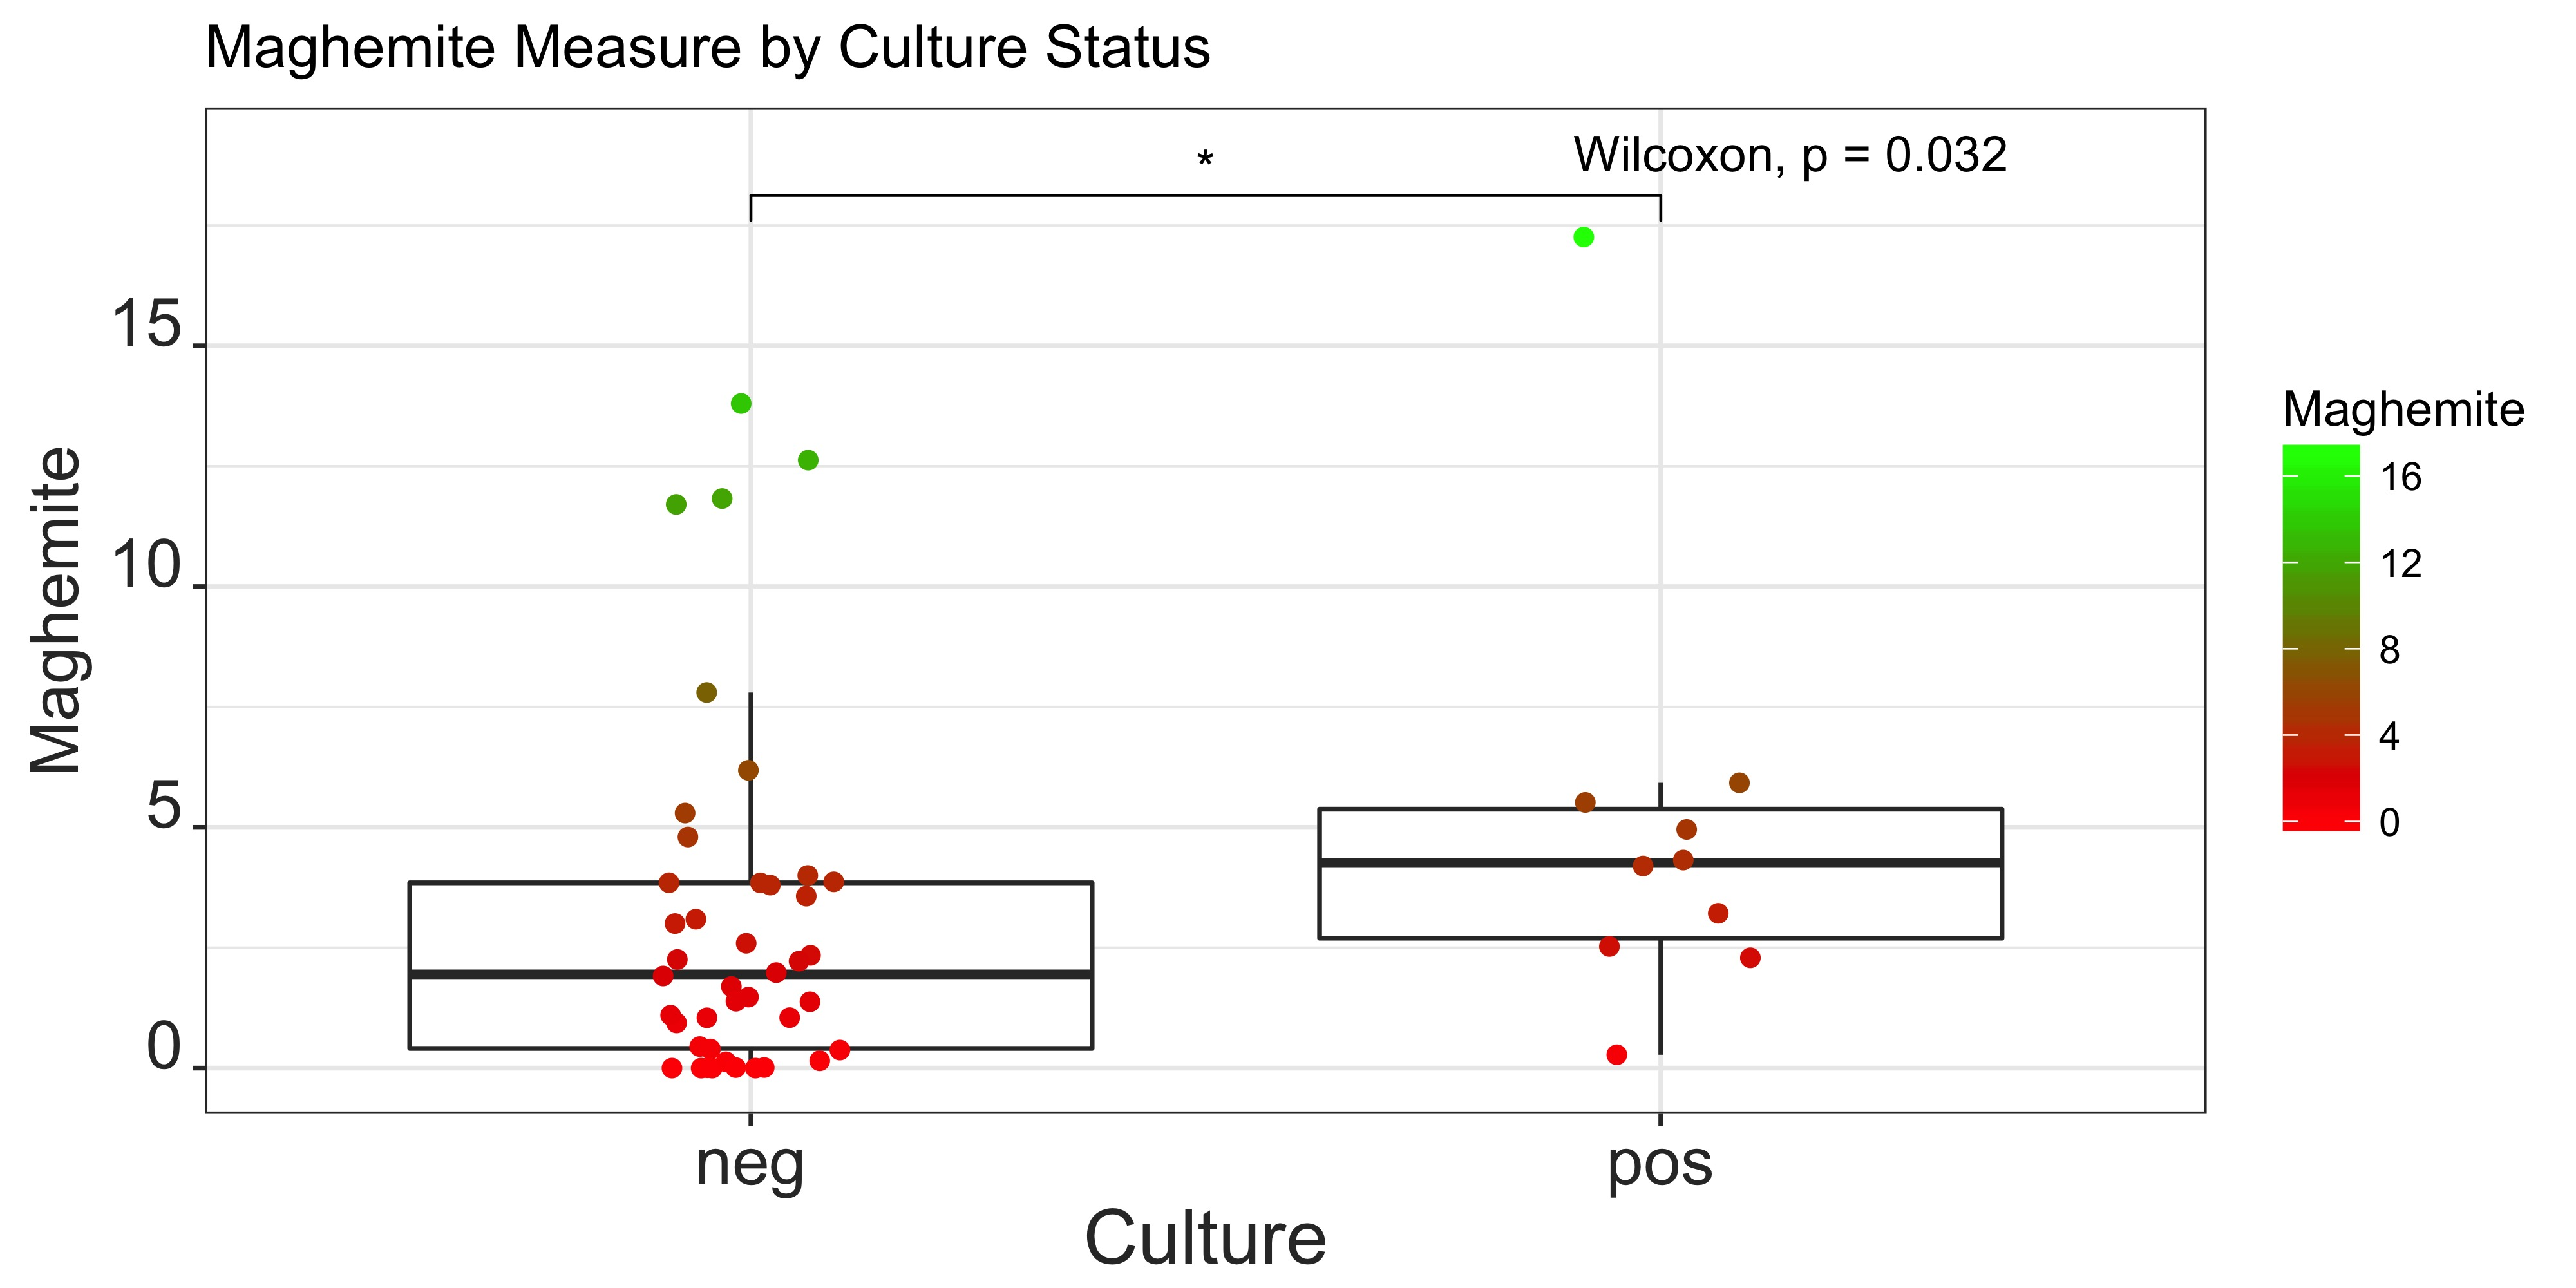
\includegraphics[height=4cm, width=5cm]{soil.jpeg}
	
	\end{block}
	\vspace{-0.5cm}
	\begin{block}{Pulmonary NTM}
	\vspace{-0.3cm}
	\begin{itemize}
	\item 90\% of NTM cultures are from respiratory samples
	\item The lung has the lowest abundance of bacteriophages among human niches
	\end{itemize}
	\end{block}
	
	
	
	\tiny{O'Brien, R., et al. American Review of Respiratory Disease 1987 \\ Aziz R., et al. Frontiers in microbiology 2015}

	
	\end{frame}
	
	
	\begin{frame}{Of "Viral" Importance}
	\begin{columns}
	\column{0.7\textwidth}
	
	\begin{block}{Bacteriophages (Phages)}
	Phages are DNA viruses that infect prokaryotes
	\end{block}
	
	\begin{block}{Bacteriophage Adherence to Mucus (BAM)}
	\begin{itemize}
	\item \alert{Phages act as an innate immune system in mucosal tissues}
	\item Prior studies identified Ig-like motifs in induced phages from Pseudomonas cultures
	\end{itemize}
	\end{block}
	\vspace{-0.3cm}
	\begin{block}{Phages in the Lungs}
	Does phage abundance in the lungs affect bacterial biofilm formation?
	\end{block}
	\vspace{0.2cm}
	\tiny{ Barr, Jeremy, et al., PNAS 2013 \\ Tariq, Mohammad, et al., Frontiers in Microbiology 2015}
	
	\column{0.4\textwidth}
	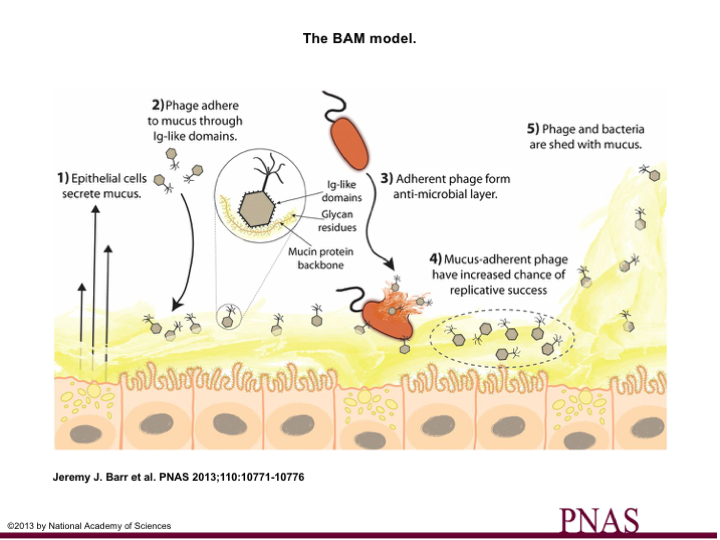
\includegraphics[height=5.5cm, width=5cm]{barr.png}
	\end{columns}

	
	
	
	\end{frame}
	
	
	\begin{frame}{Molecular Methods to Study Phages}
	\begin{columns}
	\column{0.5\textwidth}
	\begin{block}{Difficulties of phage study}
	\begin{itemize}
		\item Lack of universal marker gene
		\item Sequence heterogeneity 
		\item Misclassification in databases
	\end{itemize}
	\end{block}
		
		
	\begin{block}{Phage Isolation Methods}
	\begin{itemize}
		\item Biological filtration
		\item In silico methods
	\end{itemize}
	\end{block}
	
	\column{0.5\textwidth}
	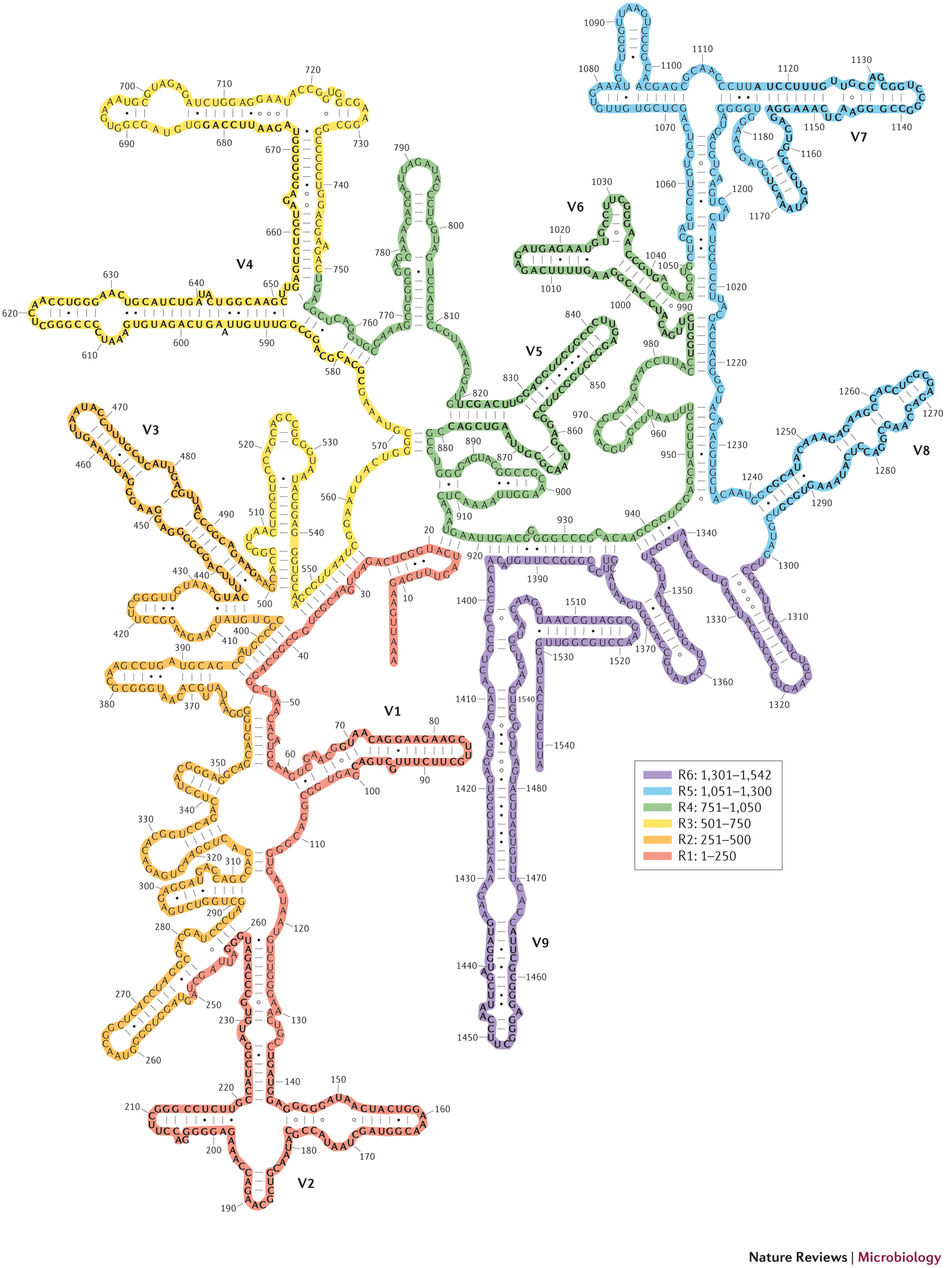
\includegraphics[height=5.5cm, width=5cm]{ribosome.jpg} \\
	\tiny{Yarza, P., et al. Nature Reviews Microbiology 2014}
	\end{columns}
		
	
	\end{frame}

	
	\begin{frame}{Objective}
	\center
	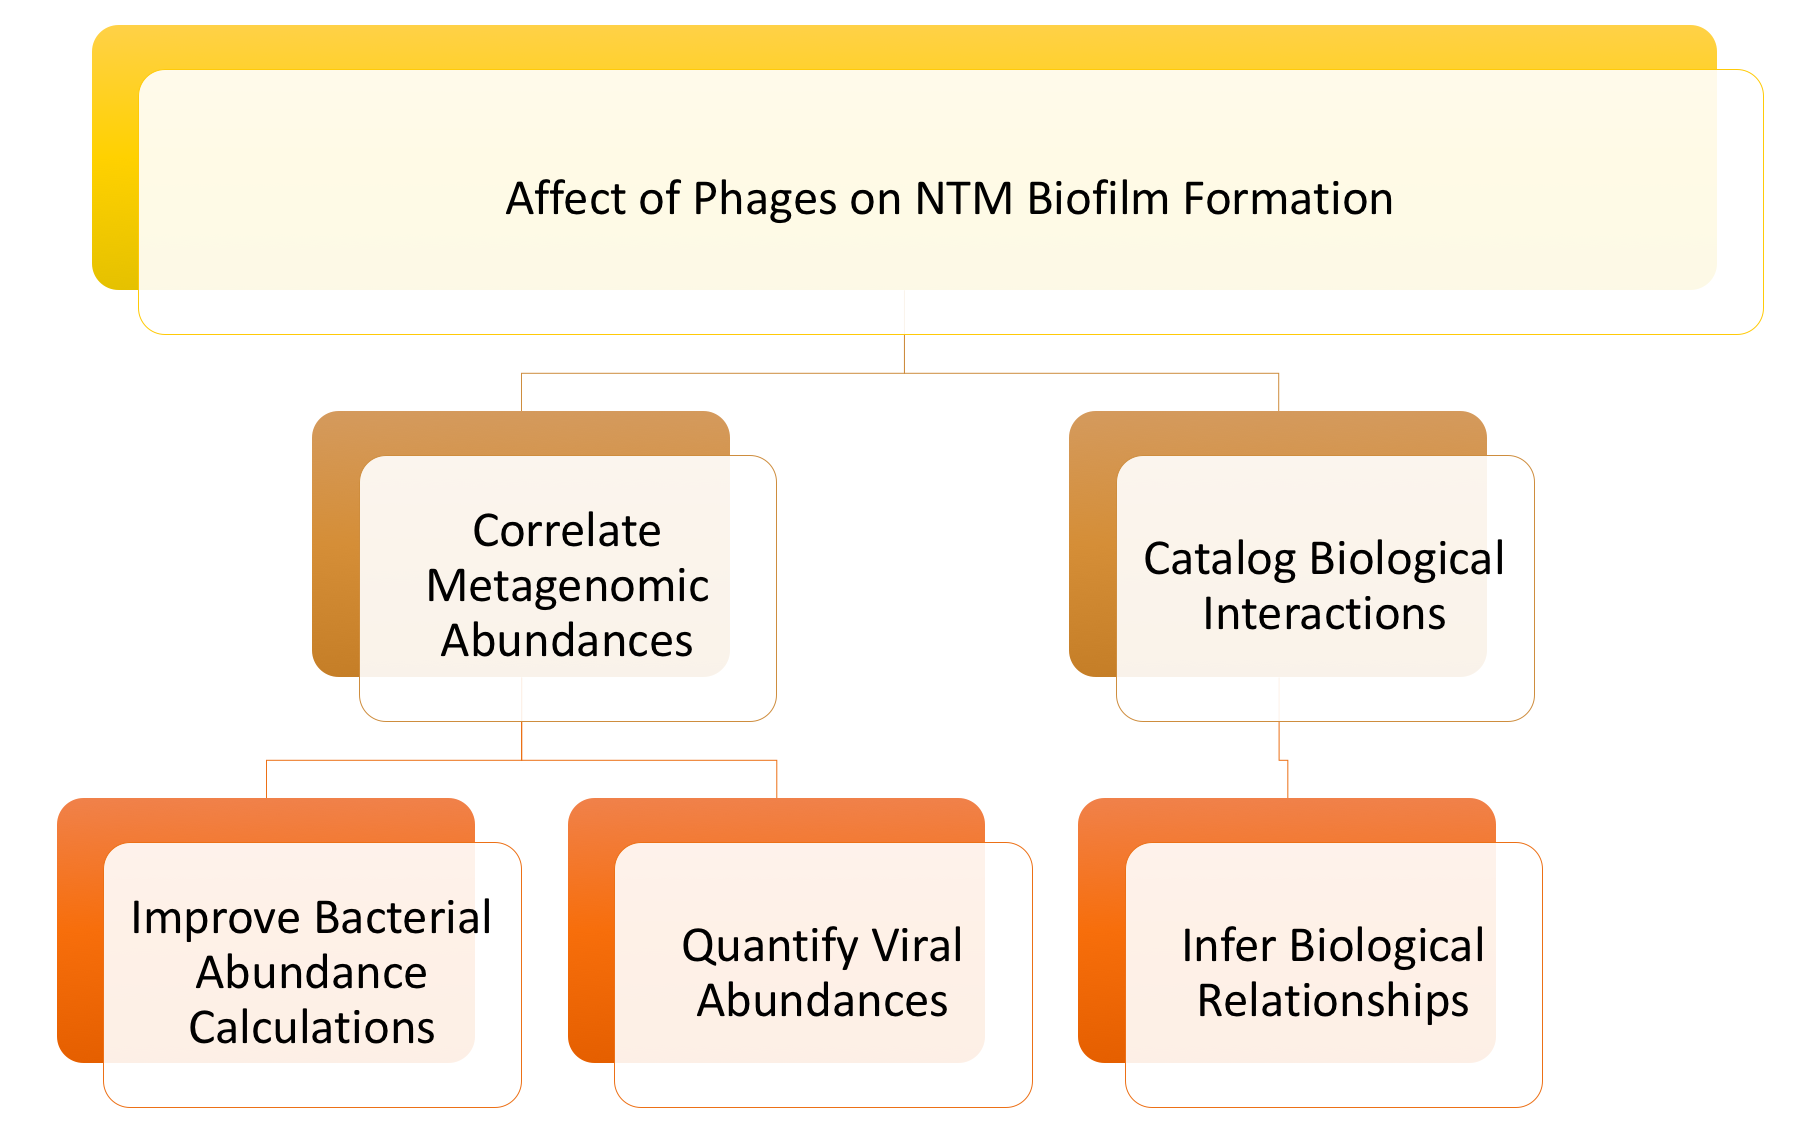
\includegraphics[height=6cm, width=9cm]{objective.png}
	
	\end{frame}


	
\section{Metagenomic Simulation Study}
\subsection{}
	\begin{frame}{Metagenomics}
	\begin{columns}
	\column{0.5\textwidth}
	\begin{block}{What is Metagenomics?}
	Unbiased study of all genetic material in a sample
	\end{block}
	\begin{block}{Importance of Metagenomics}
	\begin{itemize}
	\item Functional capabilities of a sample
	\item Species level distinctions
	\item Due to lack of a universal gene marker, phages are studied by metagenomics
	\end{itemize}
	\end{block}
	
	\column{0.5\textwidth}
	
\includegraphics[height=5.5cm, width=5cm]{mosaic.png}
	\end{columns}
	\end{frame}
	

	
	\begin{frame}{Metagenomics Gold Standard}
	
	\begin{block}{Critical Assessment of Metagenome Interpretation (CAMI)}
	\vspace{-0.3cm}
	\begin{itemize}
	\item Comprehensive simulation study of tools from all levels of analysis (binners, assemblers, taxonomic profilers) \\
	\item Viral and plasmids affected the performance of taxonomic profilers and abundance calculations
	\end{itemize}
	\end{block}
	\begin{columns}
	\column{0.5\textwidth}
	\includegraphics[height=5cm, width=5.5cm]{Filtered.png}
	\column{0.5\textwidth}
	\includegraphics[height=5cm, width=5.5cm]{unfiltered.png}
	\end{columns}
	
	\tiny{Sczyrba, A., et al. Nature Methods 2017}
	\end{frame}
	

	
	\begin{frame}{Viral Filtration Simulation Study}
	\begin{block}{Study Design}
	30 simulated mixed metagenomes are used to compare the viral contiguous sequence (contigs) identification performance of multiple tools
	\end{block}

	\begin{block}{Sequencing Depth of Experiment} 
	Each metagenome is comprised of 10 million reads
	\end{block}
	\begin{block}{Complexity of Metagenomes}
	8 bacteria and 8 phages comprise the low complexity samples in each metagenome
	\end{block}

	\end{frame}
	
	\begin{frame}{Genomes in Simulation}
	\begin{columns}
		\column{.5\textwidth}
			\begin{block}{Virus - 0.12 Mb}
			\begin{itemize}
			\item Bacillus phage Pony
			\item Caulobacter phage CcrColossus
			\item Mycobacterium phage Bxb1
			\item Mycobacterium phage Che9d
			\item Mycobacterium phage TM4
			\item Pseudomonas phage vB-PaeM-C2-10-Ab1
			\item Staphylococcus phage CNPH82
			\item uncultured phage crAssphage
			\end{itemize}
			\end{block}	
		\column{.6\textwidth}
			\begin{block}{Bacteria - 4.72 Mb}
			\begin{itemize}
			\item Bacillus subtilis subs. subtilis 168
			\item Clostridium acetobutylicum ATCC 824
			\item Clostridium perfringes str. 13
			\item Lactococcus lactis subsp. lactis Il1403
			\item Pseudomonas aeruginosa LESB58
			\item Staphylococcus aureus subsp. aureus N315
			\item Streptococcus pyogenes M1 476
			\item Xylella fastidiosa 9a5c
			\end{itemize}
			\end{block}
	\end{columns}
	\end{frame}
	
	\begin{frame}{Tools Used in Study}
	\begin{block}{Assembler}
	MEGAHIT - Effective at assembling viromes \\
	\tiny{Roux, S, et al. PeerJ 2017}
	\end{block}
	
	\begin{block}{Viral Contig Identification Methods}
	VirFinder - Viral contig K-mer identification model \\ 
	\tiny{Ren, Jie, et al. Microbiome 2017}
	
	\large{Blastx - Filtering against a viral protein database} \\
	\tiny{Camacho C., et al. BMC Bioinformatics 2008} \\
	
	\large{VirSorter - Hybrid HMM and gene marker database} \\
	\tiny{Roux, S., et al. PeerJ 2015} \\
	
	\large{vHMM - Iterative HMM trained on viral genes} \\
	\tiny{Paez-Espino, D., et al. Nature 2016} 
	
	\end{block}
	
	
	\end{frame}
	
	
	
	
	\begin{frame}{Performance Measurements}
	
	\begin{block}{True Viral Contigs}
	True viral contigs are defined by BLAST hits (E-value 10\^-05) against a custom database of the reference phages and bacterial prophage elements. 
	\end{block}
	
	\begin{block}{Term Definitions}
	\begin{columns}
	\column{.3\textwidth}
	TP = True Positive
	\column{.3\textwidth}
	FP = False Positive
	\column{.35\textwidth}
	FN = False Negative
	\end{columns}
	
	\end{block}
	\vspace{-0.2cm}
	\begin{block}{Performance Metrics}
	\begin{itemize}
	\item Recall = TP / (TP + FN)
	\item Precision = TP / (TP + FP)
	%\item F1 = (2*TP) / (2*TP + FP + FN)
	\end{itemize}
	\end{block}
	\end{frame}
	
	\begin{frame}{Recall and Precision}
	
	\begin{block}{Order of Tools}
	\tiny{from left to right}
	\center
	\large{BLAST, vHMM, VirFinder, VirSorter}
	\end{block}
	\begin{columns}
	\column{.5\textwidth}
	\center
	Recall
	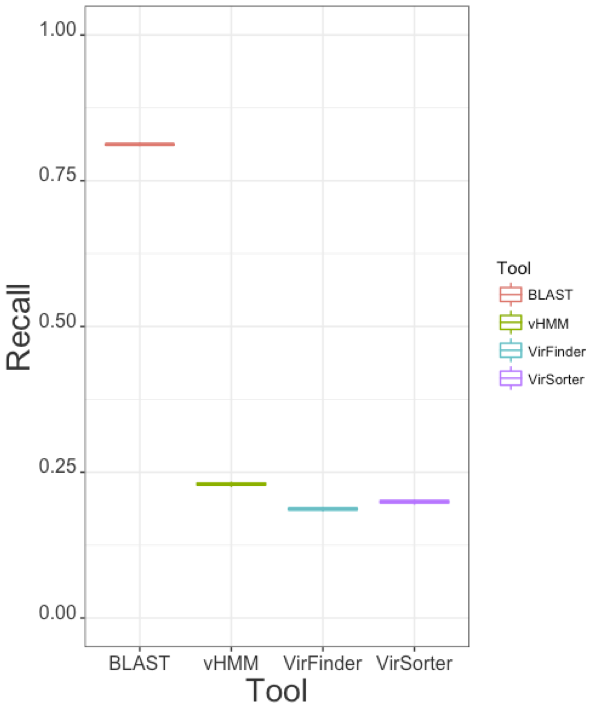
\includegraphics[height=5cm, width=6cm]{Recall.png}
	\column{.5\textwidth}
	\center
	Precision
	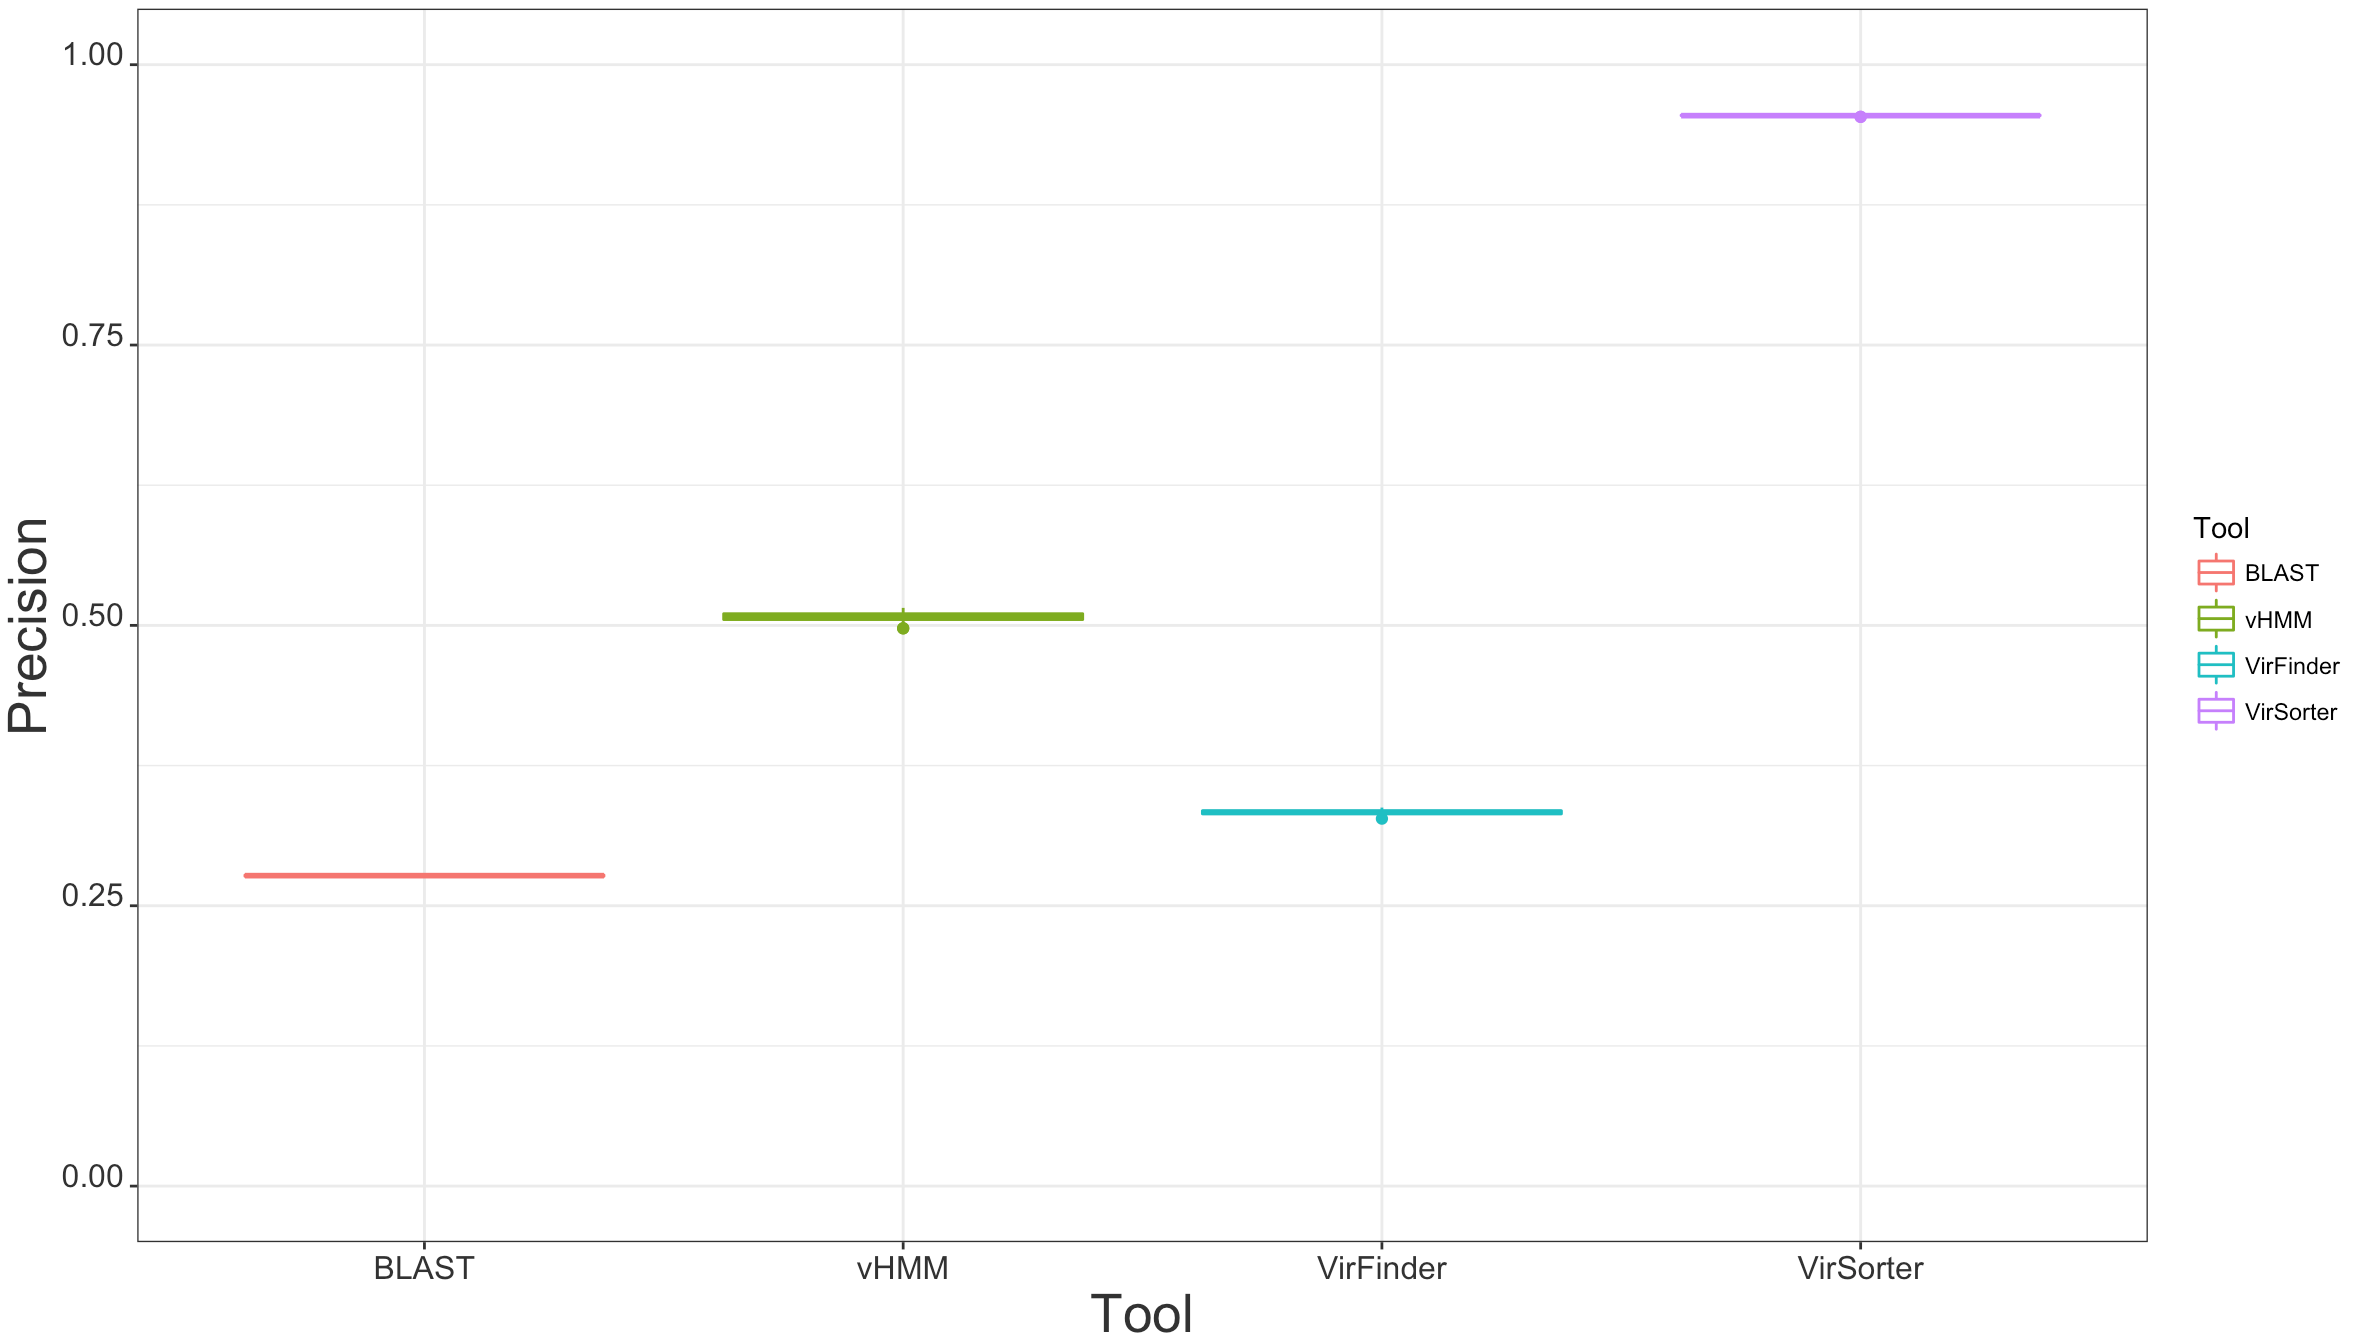
\includegraphics[height=5cm, width=6cm]{Precision.png}
	\end{columns}
	\end{frame}
	
	\begin{frame}{Conclusions}
	
	\begin{block}{Performance}
	The variance of tool performance suggests that no single tool is optimal for viral filtration
	\end{block}
	
	
	\begin{block}{Tool Parameter Optimization}
	Used default tool parameters for all tools
	\begin{itemize}
	\item Lenient BLASTX filtering resulting in false positives
	\item vHMM model is the second iteration
	\end{itemize}
	\end{block}
	
	
	\end{frame}
	
	\begin{frame}{Future Directions}
	
	\begin{block}{Expansion of Tools}
	Inclusion of binners MetaBat and MetaWatt 3.5
	\end{block}
	
	\begin{block}{Expanded Dataset}
	Filter viral elements from CAMI data
	\end{block}
	
	\begin{block}{Combinations of Tools}
	Explore how the tools perform in combinations
	\end{block}
	
	\end{frame}

\section{GRAB}
\subsection{}

	
	\begin{frame}{Creating Custom BLAST Databases}
	\begin{block}{Demand for Custom Databases}
	The Strong Lab uses custom databases to identify mycobacterium elements in metagenomics
	\end{block}
	
	\begin{block}{Current Tools}
	\begin{itemize}
	\item makeblastdb from Command-line BLAST allows users to create custom BLAST databases
	\item makeblastdb requires local sequences to create usable database
	\end{itemize}
	\end{block}
	\end{frame}
	
	\begin{frame}{Batch Sequence Retrieval}
	\begin{block}{Current Methods}
	\begin{itemize}
	\item NCBI Webserver
	\item ESearch / Efetch function
	\item biomartr R package
	\end{itemize}
	\end{block}
	
	\begin{block}{Test Case}
	Retrieve protein sequences of three Mycobacterium subspecies \\ 
	\begin{itemize}
	\item Mycobacterium avium paratuberculosis
	\item Mycobacterium abscessus massiliense
	\item Mycobacterium abscessus bolletii
	\end{itemize}
	\end{block}
	
	\end{frame}
	
	
	\begin{frame}{NCBI Webserver}
	\begin{block}{Batch Download Process}
	\begin{itemize}
	\item Query Assembly: "Mycobacterium abscessus \alert{subsp.} massiliense"[Organism] OR "Mycobacterium abscessus \alert{subsp.} bolletii"[Organism] OR "Mycobacterium avium \alert{subsp.} paratuberculosis"[Organism] 
	\item Select Complete Genome Tab
	\item Click "Download Assemblies" button and select Protein FASTA from File Type drop down 
	\end{itemize}
	\end{block}
	\begin{block}{Difficulties}
	\begin{itemize}
	\item Query string must to be specific
	\item Length of query string can become unwieldy
	\item Sparse information on download procedure and examples
	\end{itemize}
	\end{block}
	\end{frame}
	
	
	
	\begin{frame}{Efetch and biomartr}
	
	\begin{block}{Efetch Retrieval Process}
	Efetch can be utilized via Python or via command-line
	
	\texttt{handle = Entrez.efetch(db="nuccore", id= \alert{UID\_List} , rettype = "fasta\_cds\_aa")}
	
	\end{block}
	
	\begin{block}{biomartr Sequence Retrieval}
	\texttt{library(biomartr) \\
	meta.retrieval(kingdom = "bacteria", \alert{group = "Actinobacteria"}, db = "genbank", type = "proteome")}
	\end{block}
	
	\begin{block}{Difficulties}
	\begin{itemize}
	\item Entrez.efetch function requires \textit{a priori} knowledge of Entrez UID 
	\item biomartr only able to bulk download phylum level
	\item Programming skills important [not required for Efetch]
	\end{itemize}
	\end{block}
	
	\end{frame}
	
	
	\begin{frame}{Genomic Retrieval and Blast Database Creation (GRAB)}
	\begin{block}{A Batch Retrieval System for Biologists}
	Well documented command line tool and web interface (in development)
	\end{block}
	
	\begin{block}{GRABs Sequences by Taxonomy}
	\begin{itemize}
	\item GRAB requires the name of organisms and the taxonomic level 
	\item GRAB retrieves genomic, coding sequences, or protein sequences
	\end{itemize}
	\end{block}
	
	\begin{block}{GRAB Sequence Retrieval}
	\texttt{python GRAB.py -m protein -q paratuberculosis,massiliense,bolletii -l subspeices}
	\end{block}
	\end{frame}
	
	\begin{frame}{Genomic Retrieval and Blast Database Creation}
	\center
	GRAB Pipeline
	
	
	\end{frame}
	

	\begin{frame}{Demand for GRAB}

	
\includegraphics[height=1cm, width=4cm]{biostars.png} \\
	Nine questions related to bulk download of protein or genomic sequences (Over 58K views) 
	
	
\includegraphics[height=1cm, width=4cm]{stack.png} \\
	Four question related to bulk download of protein or genomic sequences (Over 3.5K views)
	
	
	\end{frame}
	
	\begin{frame}{Future Directions}
	\begin{block}{Webserver}
	Shiny web application in development
	\end{block}
	
	\begin{block}{Viral GRAB}
	\begin{itemize}
	\item Expansion of GRAB to viral elements
	\item Features include ability to filter viruses by genetic material type
	\end{itemize}
	\end{block}
	\end{frame}
	
	

\section{Building Up Domains}
\subsection{}
	
	\begin{frame}{Endogenous Viral Elements (Prophages)}
	\begin{block}{Lysogenic Life Cycle}
	Viruses can integrate into host for an extended period of time
	\center
	\vspace{-0.2cm}
	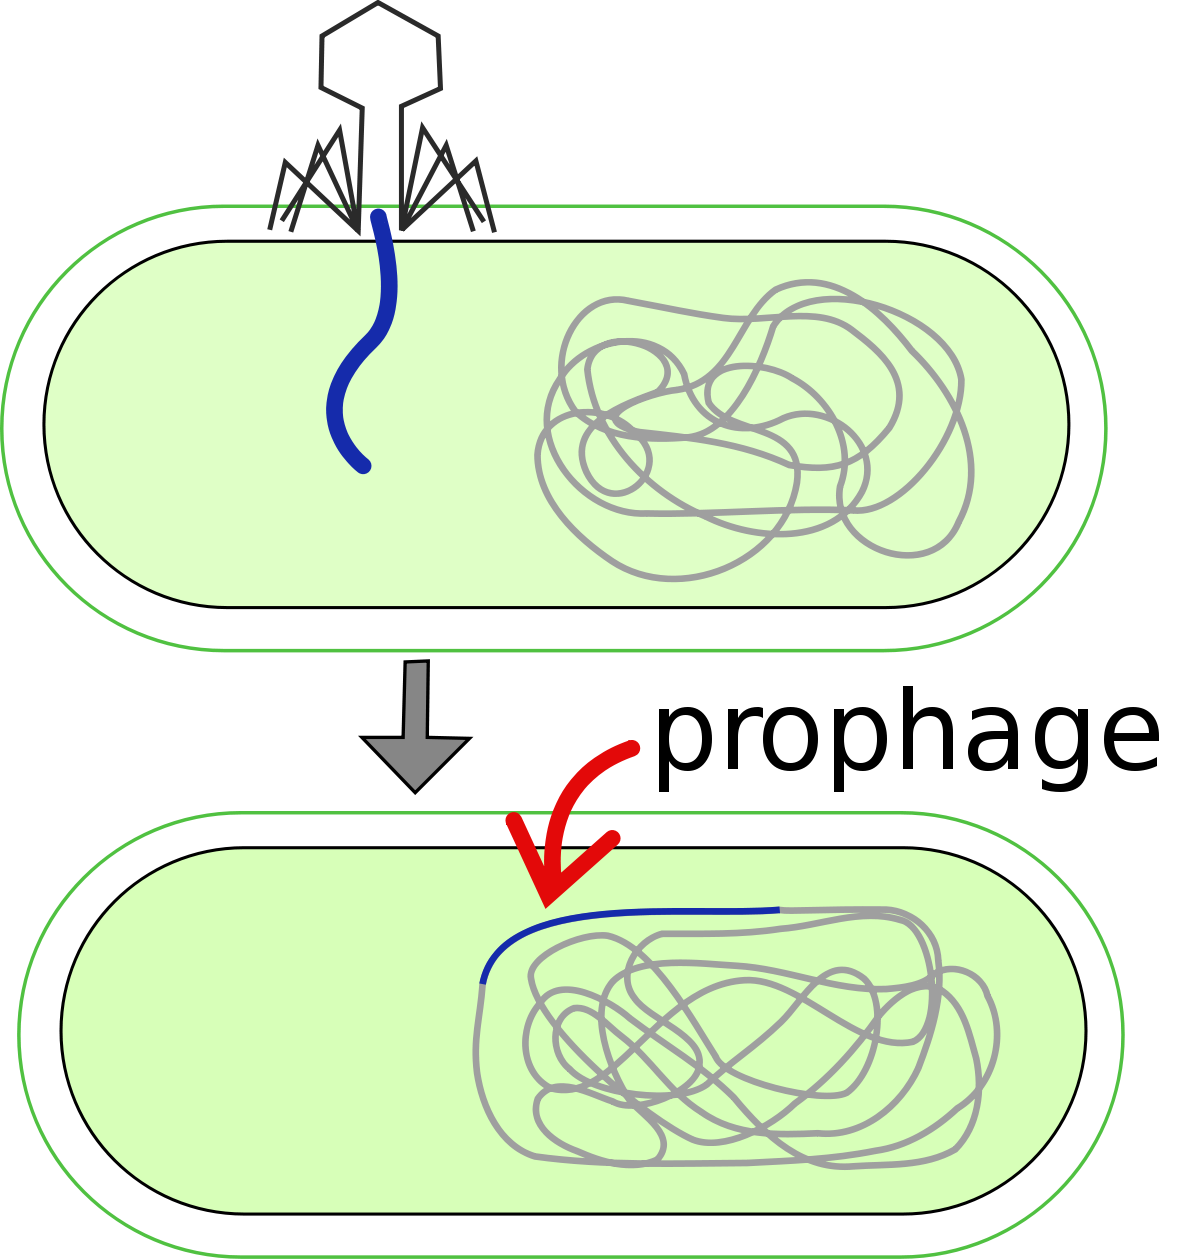
\includegraphics[height=3.5cm, width=5cm]{prophage.png}
	\end{block}
	\begin{block}{Importance of Prophages}
	Prophages can confer advantages to host improving survival \\ 
	Prophages are important to the emergence of pathogenic bacteria
	\end{block}
	
	\tiny{Canchaya C., et al. Curr Opin Microbiol 2003 \\ Wagner PL. \& Waldor MK. Infect Immune 2002}
	\end{frame}

	\begin{frame}{Finding Prophages}
	\begin{block}{Prophage Discovery Problem}
	Same difficulties as gene prediction: finding signal in data
	\center
	
\includegraphics[height=4cm, width=5cm]{dna.png}
	\end{block}
	\end{frame}
	
	\begin{frame}{Prophage Discovery Tools}
	\begin{block}{Number of Tools}
	10 tools listed at Omic Tools for prophage discovery
	\end{block}
	\begin{block}{Methods Used}
	\begin{itemize}
	\begin{columns}
	\column{0.5\textwidth}
	\item Sequence similarity
	\item Hidden Markov models 
	\item Transcription direction
	\column{0.5\textwidth}
	\item Protein length
	\item Sliding window GC content
	\item Phage specific kmer
	\end{columns}
	\end{itemize}
	\center
	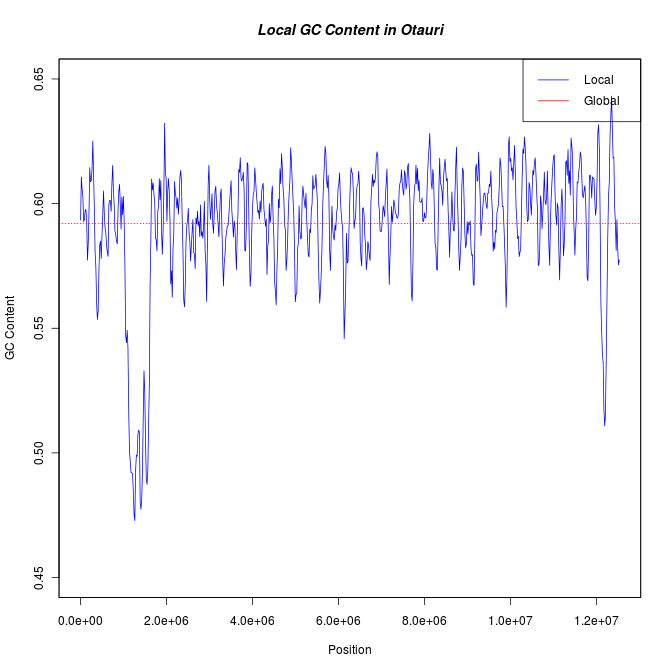
\includegraphics[height=3.5cm, width=5cm]{gc.png}
	\end{block}
	\end{frame}
	
	\begin{frame}{Prophage Discovery Methods}
	\begin{block}{Top Down Methods}
	All prophage discovery methods find prophages within contiguous sequences or genomes
	\center
	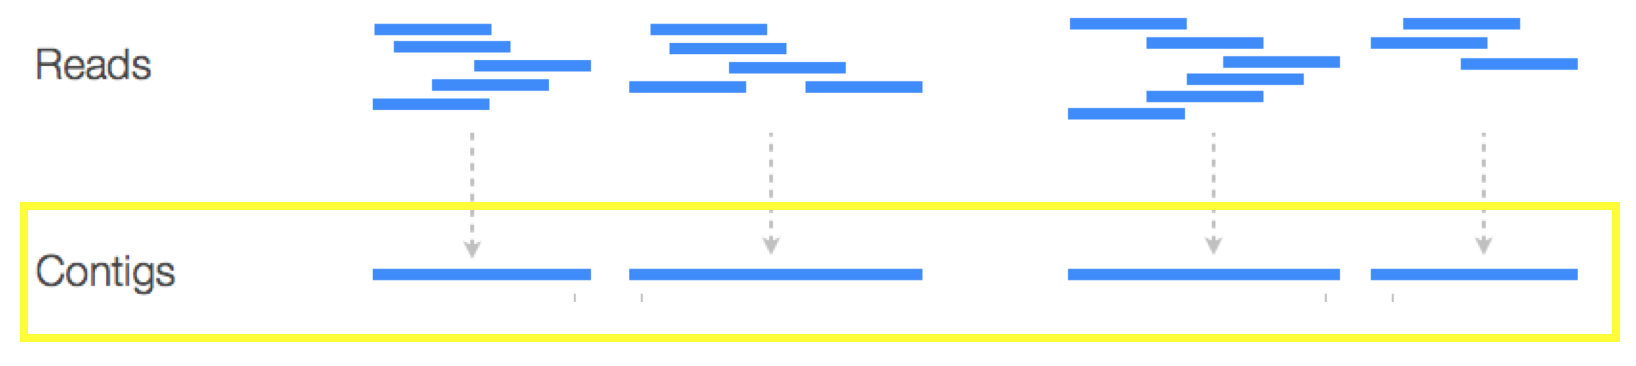
\includegraphics[height=3cm, width=5cm]{box_contigs.png}
	\end{block}
	
	
	\begin{block}{Potential Prophage Tool Pitfalls}
	\begin{itemize}
	\item Metagenomics produces short contigs that are discarded
	\item In metagenomics, prophage hosts may not be identified 
	\end{itemize}
	\end{block}
	
	
	\end{frame}
	

	
	\begin{frame}{Building Up Domains (BUD) Algorithm}
	\begin{block}{Initialization}
	\begin{itemize}
	\item Metagenomic reads are filtered by BLAST against Viral RefSeq
	\item Remaining reads are assembled into contigs
	\end{itemize}
	\end{block}
	\vspace{-0.5cm}
	\center
	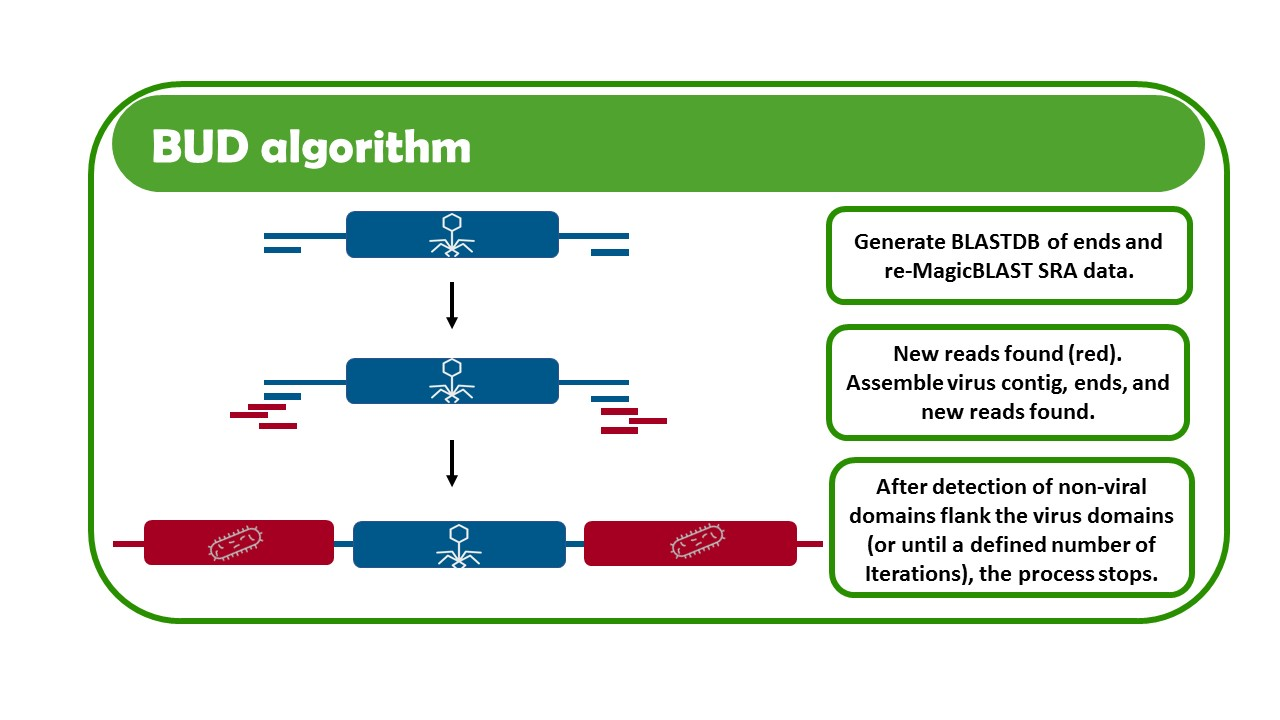
\includegraphics[height=6.75cm, width=10cm]{BUD_Algorithm.jpg}
	
	\end{frame}
	
	\begin{frame}{Potential Uses of BUD	}

	\begin{block}{Expanding Known Phage Host Range}
	BUD has the potential to identify novel hosts for prophages
	
	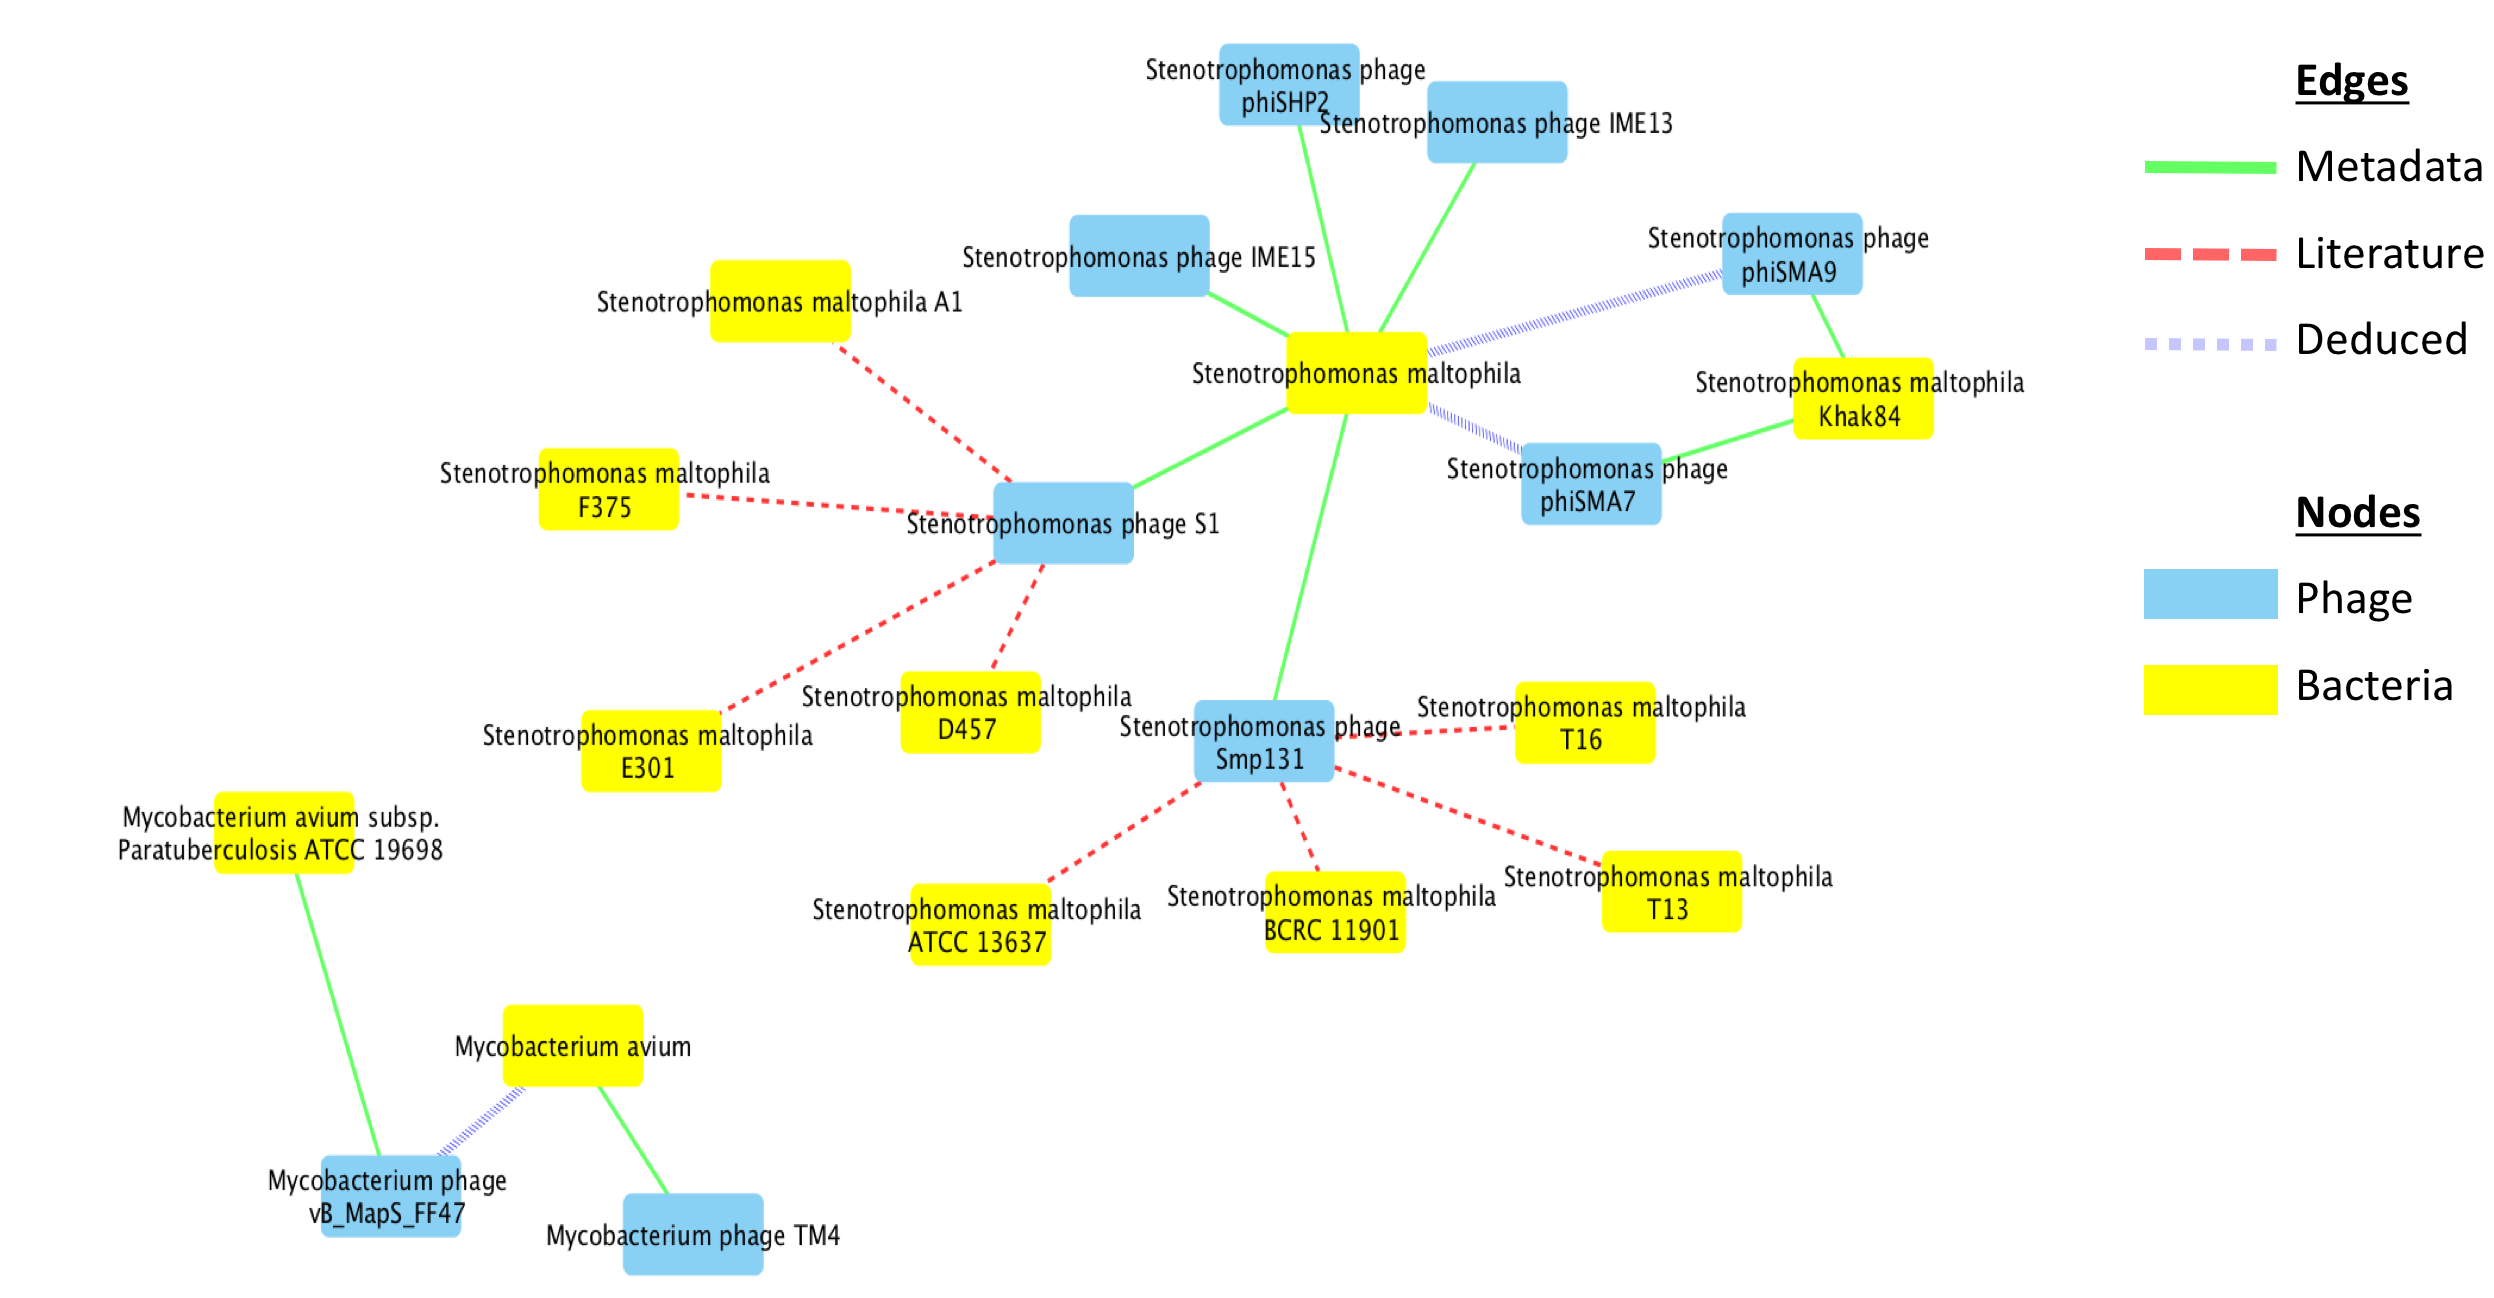
\includegraphics[height=6cm, width=11cm]{network.png}
	\end{block}
	
	\end{frame}
	
	\begin{frame}{Current Implementations of BUD}
	\begin{block}{ViruSpy}
	\begin{itemize}
	\item Originally written for NCBI Hackathon
	\item BUD Algorithm written in Perl and BASH
	\item Utilized Magic-BLAST for streaming of reads 
	\end{itemize}
	\end{block}
	
	\begin{block}{EndoVir}
	NCBI Collaborators Jan Buchman and Ben Busby \\ 
	\begin{itemize}
	\item Written in Python
	\item Implementation of BUD with Magic-BLAST
	\end{itemize}
	\end{block}
	\end{frame}
	
	\begin{frame}{Future Directions}
	\begin{block}{Magic-BLAST Streaming}
	Create a version of BUD for local metagenomic sequences 
	\end{block}
	
	\begin{block}{Testing Performance of BUD}
	Using the simulated dataset from previous study to compare the performance of identifying prophages by current tools against BUD
	\center
	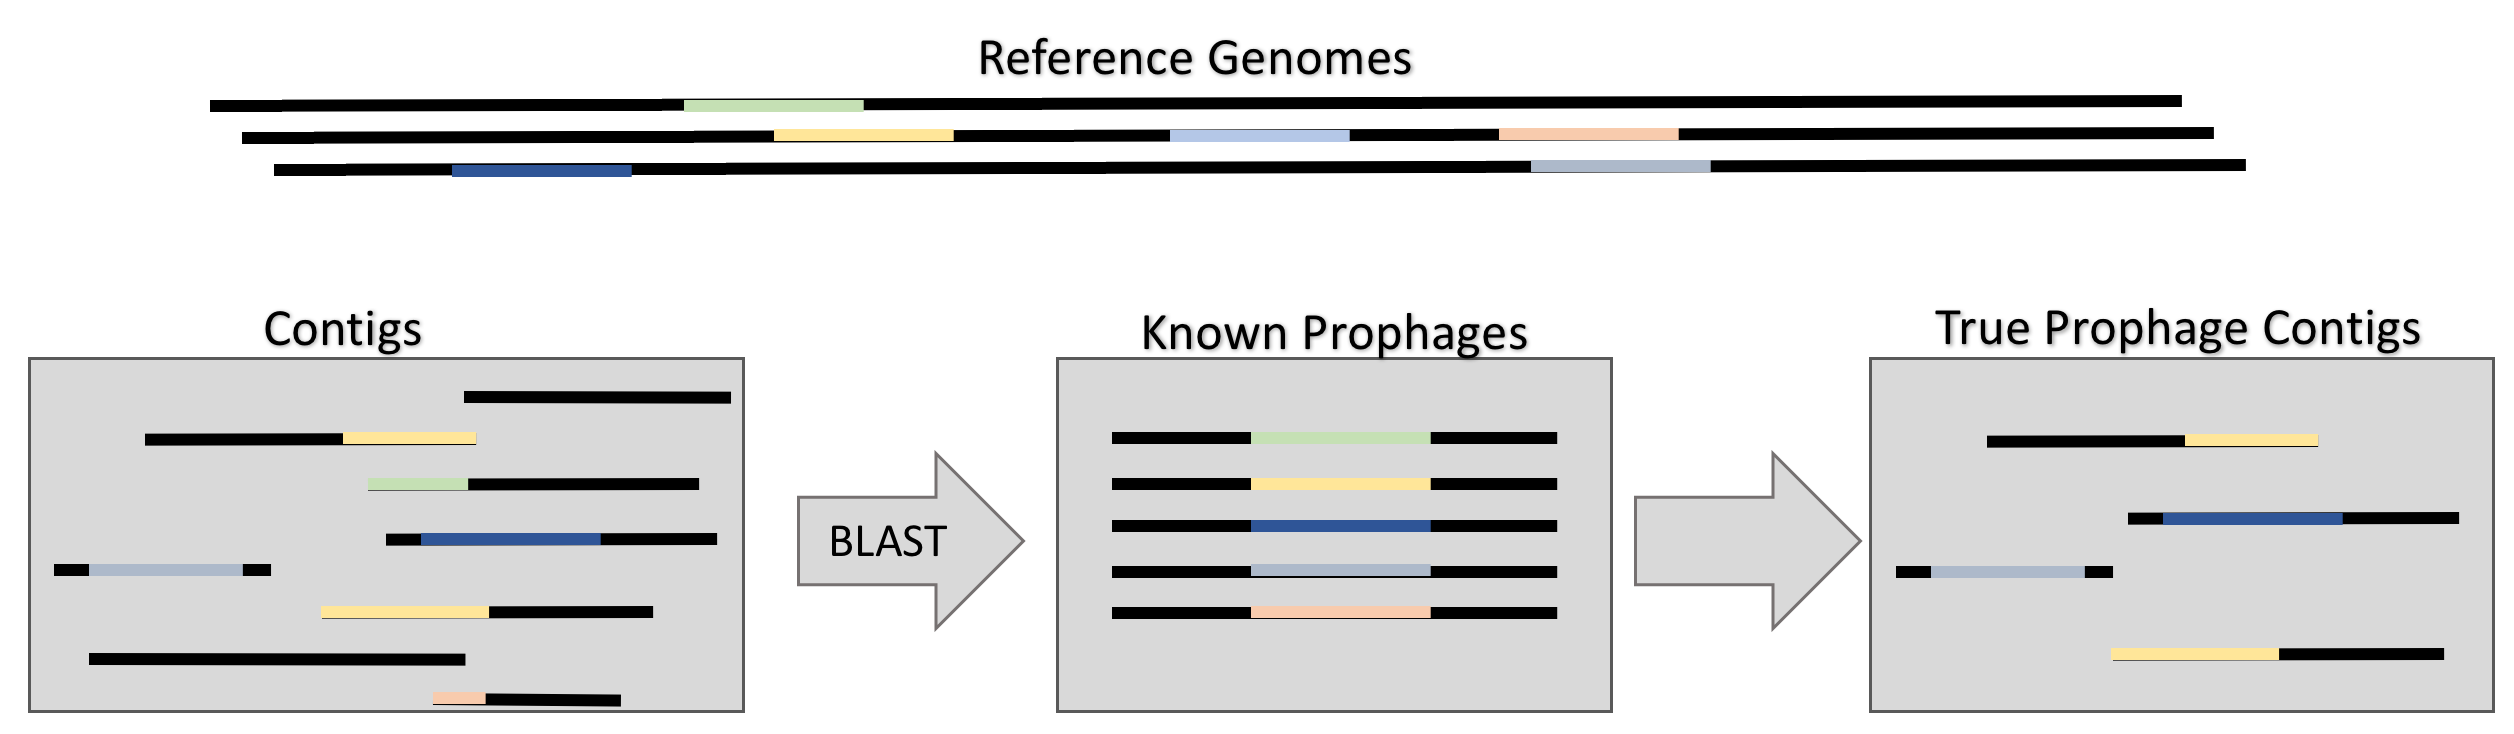
\includegraphics[height=4cm, width=8cm]{fig.png}
	
	\end{block}
	\end{frame}
	
	
	
\section{}

	\begin{frame}{Concluding Remarks}
	\center
	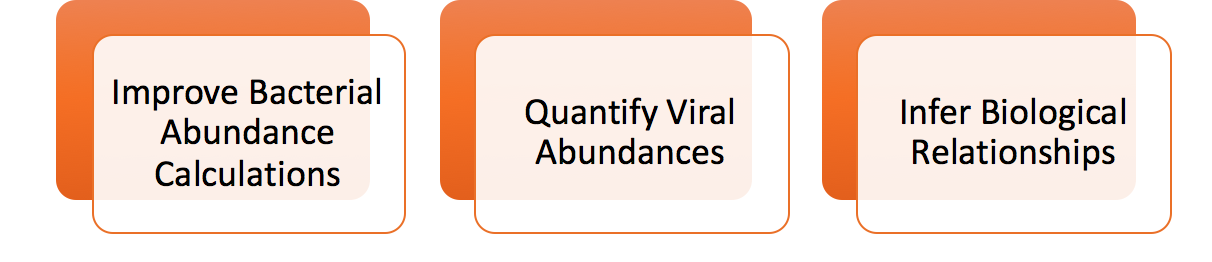
\includegraphics[height=2cm, width=10cm]{goals.png}
	\begin{columns}
	\column{0.3\textwidth}
	\begin{block}{Metagenomic Simulation Study}
	Effectively identifying viral elements improves bacterial abundance calculation
	\end{block}
	\column{0.3\textwidth}
	\begin{block}{GRAB}
	Viral GRAB will contribute to a focus on phages specific to lung infections
	\end{block}
	\column{0.3\textwidth}
	\begin{block}{Building Up Domains}
	Allows for the identification of prophages elements in metagenomics
	\end{block}
	
	\end{columns}
	
	\end{frame}
	
	
	
	
	\begin{frame}{}
	\vspace{1cm}
	{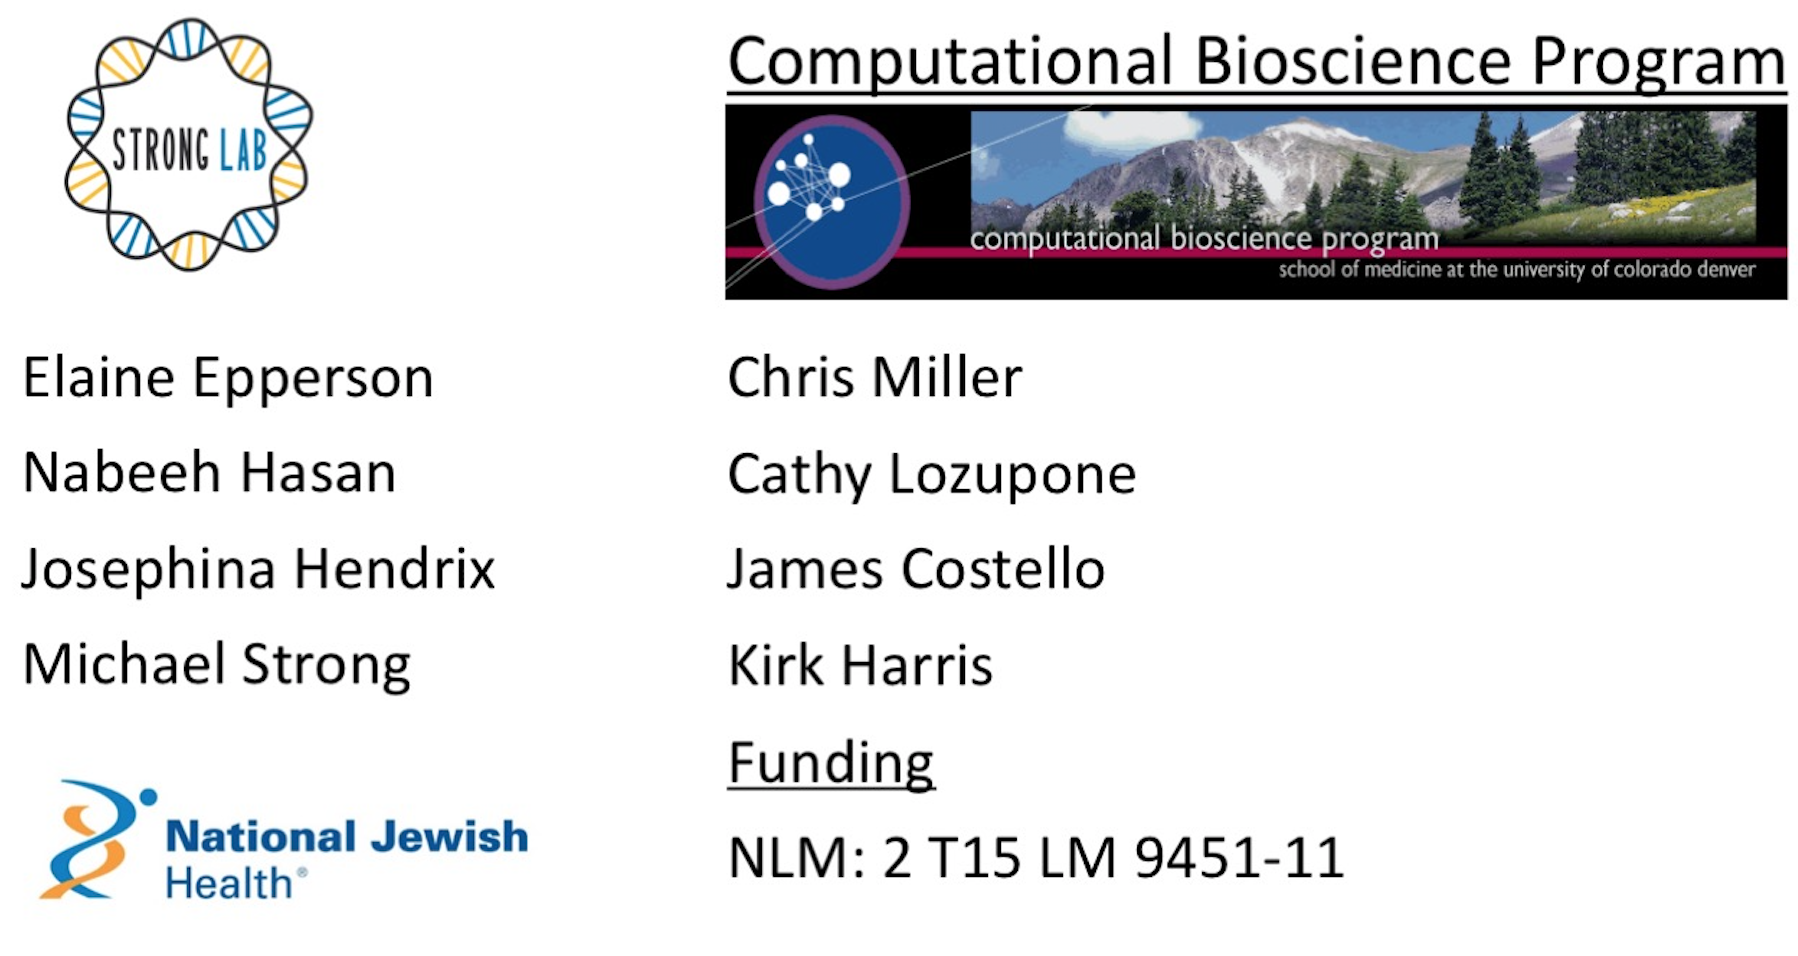
\includegraphics[height=8cm, width=11cm]{Acknowledgements.png} }
	\end{frame}
	
	
	\begin{frame}{Questions?}
	\center
	Cody Glickman \\ 
\includegraphics[height=2cm, width=2cm]{lablogo.png} \\ cody.glickman@ucdenver.edu \\ \alert{www.github.com/glickmac} \\ www.codyglickman.com
	\end{frame}
	
	
	\begin{frame}{Bias in Average Fold Coverage by GC}
	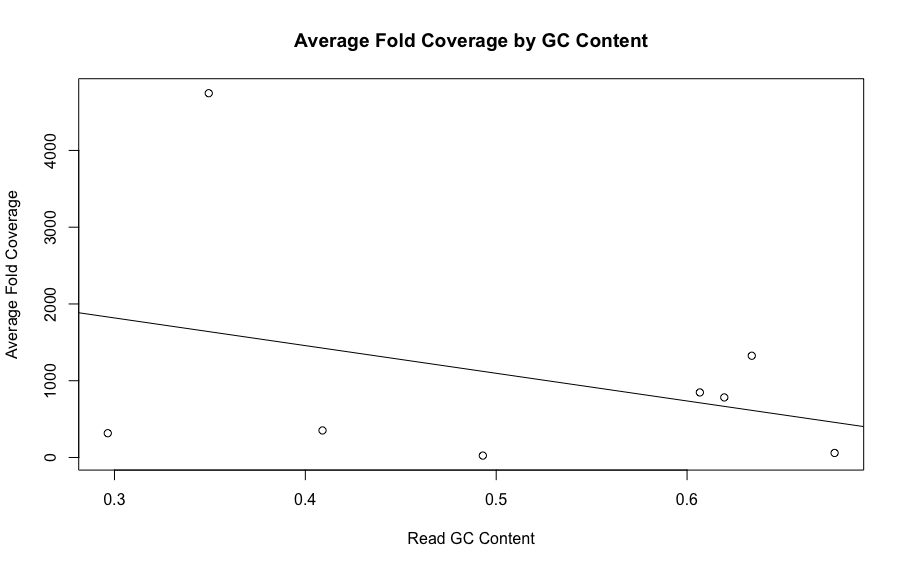
\includegraphics[height=8cm, width=11cm]{Viral_Coverage_by_GC.png}
	\end{frame}
	
	
	\begin{frame}{My Pipeline}
	\vspace{-1cm}
	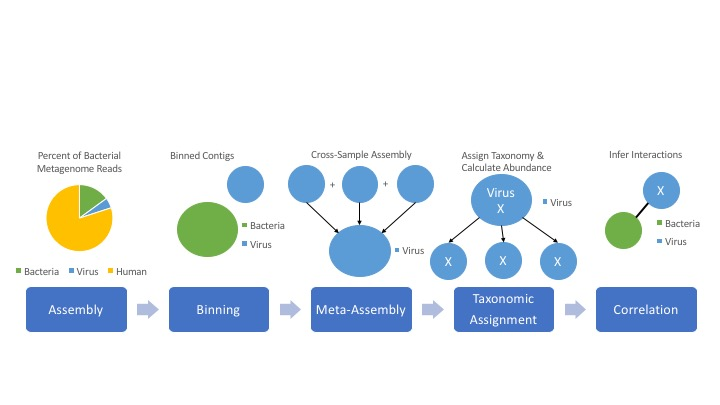
\includegraphics[height=6cm, width=11cm]{figure_2_updated.jpg}
	\end{frame}
	
	
	\begin{frame}{Tools Used in Study Continued}
	\begin{block}{Simulation Tools}
	BBMAP - a suite of tools designed for sequencing data \\
	\tiny{Bushnell, B., JGI 2016}
	\end{block}
	
	\begin{block}{Taxonomic Identification}
	Kraken - A reference-free K-mer taxonomic identifier \\
	\tiny{Wood, Derrick E., and Steven L. Salzberg Genome 2014}
	
	\large{Blastx - Referenced against a viral protein database} \\
	\tiny{Camacho C., et al. BMC Bioinformatics 2008}
	\end{block}
	
	\begin{block}{Prophage Identification}
	Phaster - A popular prophage discovery web tool  \\
	\tiny{Arndt, David, et al., Nucleic Acids Research 2016}
	\end{block}
	\end{frame}
	
	%\begin{itemize}
	%\item Prophages in bacterial reference genomes are well annotated
	%\item Location in bacterial reference genome is well annotated
	%\item find prophages in contigs and map contigs to reference.
	
	
\end{document}